\documentclass[conference,compsoc]{IEEEtran}

\usepackage[utf8]{inputenc}
\usepackage{amssymb}
\usepackage{amsthm}
\usepackage{caption}
\usepackage{cite}
\usepackage{fancyvrb}
\usepackage{graphicx}
\usepackage{hyperref}
\usepackage{xesearch}

\newtheorem{theorem}{Theorem}[section]
\newtheorem{corollary}{Corollary}[theorem]
\newtheorem{lemma}[theorem]{Lemma}

\setcounter{table}{0}
\renewcommand{\thetable}{\arabic{table}}
\renewcommand{\thefigure}{\arabic{figure}}

\usepackage{caption}
\captionsetup[table]{labelsep=period, font=footnotesize, justification=centering}
\captionsetup[figure]{name=Gambar. , labelsep=period, font=footnotesize, justification=justified}
\captionsetup[lstlisting]{labelsep=period, font=footnotesize}


% correct bad hyphenation here
\hyphenation{op-tical net-works semi-conduc-tor}


\begin{document}

\title{Perfect Queries for Non-interactive\\Ulam Searching Game with Many Lies}


% for over three affiliations, or if they all won't fit within the width
% of the page (and note that there is less available width in this regard for
% compsoc conferences compared to traditional conferences), use this
% alternative format:
% 
\author{\IEEEauthorblockN{Risyanggi Azmi Faizin\IEEEauthorrefmark{1},
Rully Sulaiman\IEEEauthorrefmark{2},
Hari Ginardi\IEEEauthorrefmark{3} and
Michał Miodek\IEEEauthorrefmark{4}}
\IEEEauthorblockA{\IEEEauthorrefmark{1}Informatics Engineering\\
Institut Teknologi Sepupuh Nopember,
Indonesia\\ Email: risyanggi@gmail.com}
\IEEEauthorblockA{\IEEEauthorrefmark{2}Informatics Engineering\\
Institut Teknologi Sepupuh Nopember,
Indonesia\\ Email: risyanggi@gmail.com}
\IEEEauthorblockA{\IEEEauthorrefmark{3}Informatics Engineering\\
Institut Teknologi Sepupuh Nopember,
Indonesia\\ Email: risyanggi@gmail.com}
\IEEEauthorblockA{\IEEEauthorrefmark{4}University of Warsaw\\
Poland\\ Email: miodziu@gmail.com}}


% make the title area
\maketitle

% As a general rule, do not put math, special symbols or citations
% in the abstract
\begin{abstract}
Pada permasalahan permainan klasik pencarian Ulam dan Rényi, penanya harus mengajukan beberapa pertanyaan iya dan tidak untuk mencari sebuah nilai antara range $[1,m]$ yang hanya diketahui penjawab, namun penjawab diperbolehkan berbohong. Sudah ada solusi dari beberapa variasi pada permasalahan pencarian Ulam dan Rényi, yaitu pada jenis query antara rentang atau subset dan jumlah maksimal bohong antara satu, dua, tiga, dan seterusnya. Namun belum ada solusi yang sempurna untuk query yang non-interaktif yaitu penjawab hanya boleh menjawab query penanya setelah penanya selesai menanyakan semua querynya. Pada paper ini akan dijelaskan solusi sempurna untuk permainan Ulam dan Rényi non-interaktif dengan maksimal kebohongan jamak menggunakan kode biner dengan jarak Hamming.
\end{abstract}

% no keywords


% For peer review papers, you can put extra information on the cover
% page as needed:
% \ifCLASSOPTIONpeerreview
% \begin{center} \bfseries EDICS Category: 3-BBND \end{center}
% \fi
%
% For peerreview papers, this IEEEtran command inserts a page break and
% creates the second title. It will be ignored for other modes.
\IEEEpeerreviewmaketitle


\section{Introduction}

\subsection{Background}

Dalam perkembangan dunia teknologi informasi selama beberapa dekade terakhir, teknologi informasi seringkali dijadikan solusi bagi permasalahan-permasalahan yang pernah ada, yang sebelumnya diselesaikan secara manual oleh manusia. Contoh permasalahan yang pernah ada adalah salah satu permasalahan klasik pencarian Rényi–Berlekamp–Ulam, atau dapat disingkat menjadi RBU. Permasalahan ini dapat diilustrasikan dengan adanya dua pemain yang disebut penanya dan penjawab. Diberikan range pertanyaan $Sm = {1,2,...,m}$. Penjawab menentukan sebuah bilangan $x \in Sm$. Penanya harus menemukan nilai $x$ dengan memberikan beberapa query khusus apakah "$x \in Q$?", dimana $Q$ adalah subset dari $Sm$, lalu penjawab menjawab "ya" atau "tidak". Permasalahan utama adalah penjawab dapat berbohong sampai $e$ kali. Tujuan dari RBU adalah mencari jumlah query minimal untuk dapat menentukan nilai $x$. 

Sudah ada beberapa variasi pada permasalahan RBU. Pelc (1987) menyelesaikan permasalahan RBU dengan query rentang $[a,b]$ dan dengan maksimal jumlah bohong adalah satu. Mundici et all (1997) dan Min et all (2016) menyelesaikan permasalahan RBU dengan query rentang $[a,b]$ dan dengan maksimal jumlah bohong dua. Ahlswede (2008) mengilustrasikan permasalah RBU dengan maksimal bobot bohong adalah $e$, dengan menggunakan \textit{bipartite graph} untuk menyimpan kanal kebohongan dan memberikan batasan asimtotik yang ketat untuk jumlah query yang dibutuhkan untuk memecahkan masalah ini.

Salah satu variasi permasalahan RBU yang diangkat dalam penelitian ini adalah pencarian Ulam dengan $m$ query subset ${q_1,q_2,...,q_m} | q_i \in Sm$, maksimal bohong adalah $e$, dan penjawab hanya boleh menjawab query penanya setelah penanya selesai menanyakan semua query-nya. Belum ada penelitian yang menyelesaikan permasalahan ini. Oleh karena itu penelitian ini bertujuan untuk memberikan solusi pada permasalahan ini.

Penelitian tentang permasalahan Ulam selama ini hanya membahas tentang query yang interaktif dari penanya dan penjawab, baik dengan jumlah maksimal bohong satu, dua, tiga, dan lebih dari tiga. Namun belum ada jurnal ilmiah yang membahas permasalahan Ulam dengan query non-interaktif dengan jumlah bohong lebih dari dua. Kontribusi dari penelitian ini adalah menggunakan metode pencarian biner non-interaktif untuk menyelesaikan permasalahan Ulam.

% You must have at least 2 lines in the paragraph with the drop letter
% (should never be an issue)

\subsection{Related work}
Subsection text here.


\section{Problem formulation}

Penjawab menentukan sebuah bilangan $x$ pada rentang $Sm=[1,n]$. Penanya harus mencari nilai $x$ dengan memberikan maksimal m query khusus apakah "$x \in Q$?", lalu penjawab menjawab "ya" atau "tidak" pada setiap query yang ditanyakan. Permasalahan utama adalah penjawab dapat berbohong sampai $e$ kali. Selain itu, penjawab hanya boleh menjawab query penanya setelah penanya selesai menanyakan semua query-nya. Tujuan dari RBU adalah mencari jumlah query minimal untuk dapat menentukan nilai $x$.

Bentuk dari query adalah string $s_1s_2s_3...s_n$ dimana si bernilai '0' atau '1'. Jawaban dari penjawab adalah "Ya" jika $s_x=1$ atau "Tidak" jika $s_x=0$ dengan asumsi penjawab menjawab jujur.

Tugas sesungguhnya dari permasalahan ini adalah bukan untuk mencari nilai $x$, tapi hanya menyiapkan query yang dapat memeungkinkan untuk mendapatkan nilai $x$ dari semua kemungkinan jawaban dari penjawab. Penjawab tidak akan menjawab query yang diberikan penanya. Jika penjawab menemukan ada suatu set jawaban yang menyebabkan lebih dari satu kemungkinan nilai $x$, maka pengujian dianggap gagal.

\begin{figure}
\centering
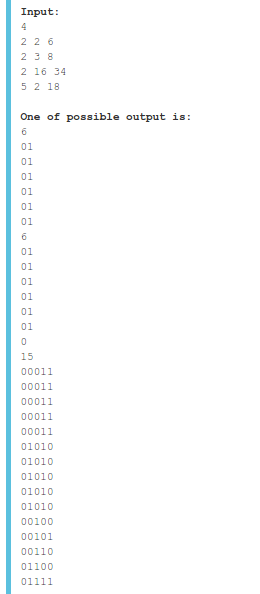
\includegraphics[scale=0.6]{../img/example.png}
\caption{Contoh kasus uji pada GUESSN5}
\label{fig:guessn5_test_case}
\end{figure}

Gambar \ref{fig:guessn5_test_case} adalah contoh empat uji kasus dari permasalahan SPOJ GUESSN5. Pada uji kasus yang pertama hanya terdapat dua angka. Penjawab dapat menjawab "YYYYYY" atau "NNNNNN" jika penjawab tidak berbohong. Penjawab dapat menjawab "YYYYYN", "YYYYNY", "YYYNYY", "YYNYYY", "YNYYYY", "NYYYYY", "NNNNNY", "NNNNYN", "NNNYNN", "NNYNNN", "NYNNNN", atau "YNNNNN" jika penjawab berbohong satu kali. Penjawab dapat menjawab "NNNNYY", "NNNYNY", "NNNYYN", "NNYNNY", "NNYNYN", "NNYYNN", "NYNNNY", "NYNNYN", "NYNYNN", "NYYNNN", "YNNNNY", "YNNNYN", "YNNYNN", "YNYNNN", "YYNNNN", "NNYYYY", "NYNYYY", "NYYNYY", "NYYYNY", "NYYYYN", "YNNYYY", "YNYNYY", "YNYYNY", "YNYYYN", "YYNNYY", "YYNYNY", "YYNYYN", "YYYNNY", "YYYNYN", atau "YYYYNN" jika penjawab berbohong dua kali. Kemungkinan jawaban selain tersebut di atas tidak mungkin karena penjawab akan berbohong tiga kali.

Pada uji kasus yang kedua penjawab mencoba memberikan solusi namun jawabannya salah. Penanya dapat menjawab "YYYNNN" yaitu jawaban yang valid karena jumlah bohong tiga kali untuk kedua kemungkinan angka. Pada kasus ini, penanya membutuhkan query tambahan.

Pada uji kasus yang ketiga penanya tidak memberikan solusi.

Pada uji kasus yang keempat penanya memberikan query yang lebih sedikit dari jumlah query maksimal yang diperbolehkan. Dari semua kemungkinan jawaban penjawab, pasti hanya ada satu jawaban nilai $x$, jadi solusi penanya berhasil.

\begin{itemize}
  \item Batas maksimum kasus uji adalah $2^7$.
  \item Interval bilangan yang yang dicari berada pada $[1,n]$, dengan n maksimum $2^12$.
  \item Dataset yang digunakan adalah dataset pada permasalahan SPOJ GUESSN5.
\end{itemize}


\section{Backround from coding theory}

Tujuan utama dari teori pengkodean (\textit{coding theory}) adalah bagaimana mengirimkan pesan pada kanal yang mengandung derau (\textit{noisy channel}) **[1]**. Misal jika ada delapan macam kata pesan yang akan dikirim, maka kita merepresentasikan pesan tersebut menjadi bitstring dengan panjang 3. Namun jika pesan tersebut dikirm langsung melewati kanal yang mengandung derau, bisa jadi misalkan ada 1 bit akan tertukar, misal $001$ menjadi $011$. Jika terjadi seperti itu, maka sebuah kata dapat tertukar menjadi kata yang lain.

Kita tahu bahwa jika kode biner sepanjang $n$ digunakan untuk membuat $2^n$ bitstring tidak dapat mendeteksi eror. Ide yang paling mungkin adalah pengirim dan penerima menyetujui sebuah metode enkripsi bitstring menjadi bitstring yang lebih panjang dan dapat mendeteksi maksimal sebanyak $e$ error.

\begin{equation}
d_H(x,y) = |\{i \in {1,...,n} \mid x_i \neq y_i\}|
\label{eq:dh}
\end{equation}

Jarak Hamming dari bitstring $x$ dan $y$ dengan panjang $n$ didefinisikan dengan persamaan \ref{eq:dh} **[2]**. Sebagai contohnya $d_H(0000,1111)= 4$ dan $d_H(00110,00101)= 2$. $d_H(x,y)$ juga dapat dikatakan jumlah minimal untuk mentransformasi dari $x$ ke $y$. Contoh $x=00110$ dan $y=00101$ memiliki perbedaan pada 2 bit terakhir dengan jarak Hamming 2, dapat dikatakan $x+00011 = y$.

\begin{equation}
wt(x) = |\{i \in {1,...,n} \mid x_i \neq 0\}|
\label{eq:wt}
\end{equation}

Bobot dari bitstring $x$ didefinisikan dengan $wt(x)$, yaitu jumlah digit pada $x$ yang bukan $0$ seperti pada persamaan \ref{eq:wt}. Sebagai contohnya, $wt(00101) = 2$ dan $wt(11111) = 5$. Jika dihubungkan dengan jarak Hamming, jika $x+e = y$ maka $d_H(x,y) = wt(x+y)$.

Terdapat sebuah sifat pada jarak Hamming yang bernama segitiga pertidaksamaan (\textit{triangle inequality}), yaitu $d_H(x,y) <= d_H(x,z) + d_H(y,z)$ untuk semua $x$, $y$, dan $z$. Dari segitiga pertidaksamaan tersebut, misalkan $z$ adalah string biner yang berisi semua $0$, maka didapatkan $d_H(x,y) <= wt(x) + wt(y)$.

Kode biner (\textit{binary code}) adalah sejumlah $M$ bitstring biner dengan panjang masing-masing bitstring adalah $n$ dan jarak Hamming pada masing masing bitstring adalah $d$. Mari kita ambil contoh $M=8$, $n=6$, dan $d=3$ pada **Kode sumber 1**. Parameter pada kode ini adalah $(6,8,3)2$, yaitu kode biner yang ditunjukkan pada angka 2, panjang bitstring 6, berisi 8 bitstring, dengan jarak Hamming minimal 3. Bitstring pada kode biner selanjutnya disebut kata kode (\textit{codeword}).


\begin{figure}
\centering
\begin{BVerbatim}
000000  100110
001011  101101
010101  110011
011110  111000
\end{BVerbatim}
\caption{Kode biner $(6,8,3)2$}
\label{fig:binarycode683}
\end{figure}


Dengan kode biner $(6,8,3)2$ pada gambar \ref{fig:binarycode683}, pengirim dan penerima menyepakati hanya kata kode yang akan dikirim dan diterima. Dengan asumsi hanya ada satu bit yang dapat error, pesan error tetap dapat dikembalikan ke bentuk semula. Misal $111100$ menjadi $111000$, $000011$ menjadi $001011$, dan seterusnya. Jarak Hamming antara setiap dua kata kode yang berbeda adalah 3, berarti dari setiap kata kode, terdapat sejumlah bitstring selain kata kode berjarak 1.

\begin{figure}
\centering
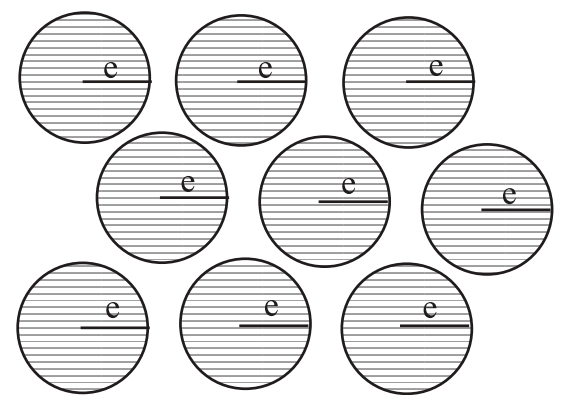
\includegraphics[width=\linewidth]{../img/codewordsball.png}
\caption{Bola codeword yang tidak saling overlap}
\label{fig:codewordsball}
\end{figure}

Notasi umum kode biner adalah $(n,M,d)2$. Kita bisa asumsikan ada $M$ bola yang tidak saling bersinggungan atau berpotongan, dengan radius bola $e=(d-1)/2$ seperti pada gambar \ref{fig:codewordsball}. Dari ilustrasi bola-bola tersebut dapat disimpulkan bahwa jika dikirimkan sebuah kata kode, bitstring setelah terjadi maksimal $e$ pertukaran bit, hasil tetap hanya dekat dengan satu kata kode saja.


\section{Solusi permainan Ulam non-interaktif}

Diberikan sebuah matriks $L$ berukuran $n \times M$ berisi $n$ query $Q\in{q_1,q_2,...,q_n} \mid qi\in{s_1,s_2,...,s_M} \mid s_i\in{0,1}$. Diberikan sebuah vektor $z \in {z_1,z_2,...,z_n} \mid z_i\in{0,1}$ berisi jawaban dari seluruh query secara berurutan, $z_i$ adalah jawaban dari $qi$, dimana $0$ berarti 'tidak' dan $1$ berarti 'ya'. Karena jika jawaban $0$ berarti query harus ditambah dengan 1 dan jika jawaban $1$ berarti query ditambah dengan 0 (diabaikan), maka kita memiliki $z'$ yaitu inverse dari $z$. 

Matriks $L'$ berukuran $M \times n$ adalah hasil transpose dari matriks $L$. Tambahkan seluruh baris pada $L'$ dengan $z'$. Maka jawaban dari permainan Ulam non-interaktif adalah index dari baris $r$ pada $L'$ yang memiliki bobot $wt(r) > n-e$.

Penanya memenangkan permainan jika $L'$ memiliki paling banyak satu row dengan $wt(x) \ge n-e$. Jika hanya ada satu row, maka row tersebut adalah jawaban permainan. Jika tidak ada satu row pun yang memenuhi, penanya tetap memenangkan permainan karena penjawab melakukan kecurangan, melakukan bohong untuk semua angka lebih dari batas yang ditetapkan.

Untuk meyakinkan bahwa setelah seluruh jawaban $z$ diberikan dan diaplikasikan ke matrix $L$ dan tidak pasti hanya ada 1 baris yang memiliki nilai $1$ antara $n-e \le wt(r) \le n$, adalah dengan memastikan bahwa jarak Hamming setiap row yang berbeda pada $L'$ adalah minimal $2*e+1$.

\begin{lemma}
Diketahui integer $n$, $M$, dan $d$. Buktikan bahwa jika $L'$ adalah kode biner $(n,M,d)2$ yang valid, maka pasti hanya ada paling banyak satu codeword c yang memiliki $0 \le wt(c) \le e$.  
\end{lemma}

\begin{proof}
(1) Jika $wt(c) = 0$ maka
\[d_H(c,x_i) >= d \mid c != x_i \mid x_i \in L'\]
\[wt(c + x_i) \ge d\]
\[wt(x_i) \ge d\]

(2) Jika $wt(c) = e$ maka
\[d_H(c,x_i) \ge d \mid c != x_i \mid x_i ∈ L'\]
\[wt(c+x_i) \ge d\]
\[wt(c) + wt(x_i) \ge wt(c+x_i) \ge d\]
\[wt(c) + wt(x_i) \ge d\]
\[e + wt(x_i) \ge d\]
\[wt(x_i) \ge d - (d-1)/2\]
\[wt(x_i) \ge (d+1)/2\]

Jadi jika ada codeword $c \mid 0 \le wt(c) \le e$ maka $wt(x_i) > e \mid x_i \neq c$.
\end{proof}

Dari pembuktian diatas, dapat disimpulkan bahwa untuk menyelesaikan permainan pencarian Ulam non-interaktif dengan batas pencarian $M$ dan maksimal kebohongan $e$, transpose dari $n$ query yang dibuat harus membentuk kode biner $(n,M,d)2$.

\begin{lemma}
Diketahui integer $n$, $M$, dan $d$. Buktikan bahwa jika $L'$ adalah kode biner $(n,M,d)2$ yang valid, maka jika setiap codeword $c$ pada $L'$ ditambah dengan $z \mid z \in \mathbb{F}_2^n$ maka hasilnya akan tetap menjadi kode biner $(n,M,d)2$ yang valid.  
\end{lemma}

\begin{proof}
Jika $d_H(x_i,y_i) \ge d \mid i \neq j \mid x_i,y_i \in L'$ maka
\[d_H(x_i+z,y_i+z) \ge d\]
\[wt(x_i+y_i+z+z) \ge d\]
\[wt(x_i+y_i) \ge d\]
\[d_H(x_i,y_i) \ge d\]
Jadi jika $d_H(x_i,y_i) \ge d$ maka $d_H(x_i+z,y_i+z) \ge d$.
\end{proof}

% trigger a \newpage just before the given reference
% number - used to balance the columns on the last page
% adjust value as needed - may need to be readjusted if
% the document is modified later
%\IEEEtriggeratref{8}
% The "triggered" command can be changed if desired:
%\IEEEtriggercmd{\enlargethispage{-5in}}

% references section

% can use a bibliography generated by BibTeX as a .bbl file
% BibTeX documentation can be easily obtained at:
% http://mirror.ctan.org/biblio/bibtex/contrib/doc/
% The IEEEtran BibTeX style support page is at:
% http://www.michaelshell.org/tex/ieeetran/bibtex/
%\bibliographystyle{IEEEtran}
% argument is your BibTeX string definitions and bibliography database(s)
%\bibliography{IEEEabrv,../bib/paper}
%
% <OR> manually copy in the resultant .bbl file
% set second argument of \begin to the number of references
% (used to reserve space for the reference number labels box)
\begin{thebibliography}{3}

\bibitem{IEEEhowto:kopka}
H.~Kopka and P.~W. Daly, \emph{A Guide to \LaTeX}, 3rd~ed.\hskip 1em plus
  0.5em minus 0.4em\relax Harlow, England: Addison-Wesley, 1999.

\end{thebibliography}



% that's all folks
\end{document}


